\chapter{Motivation}\label{ch:motivation}
 This chapter accounts for the motivation behind source extraction from an Electroencephalography (EEG). The concept of EEG is introduced along with its application. The potential and importance of source extraction are considered and related to the hearing aid industry. The commonly applied mathematical model for EEG measurements is presented. Currently applied methods for source extraction are considered leading to a presentation of the current state of the art methods which succeeds to overcome the limitations of previous methods. Lastly the contribution provided in this thesis is presented.          

%This chapter examines existing literature concerning source recovery from Electroencephalography (EEG) measurements. 
%At first a motivation for the source recovery problem is given, considering the application within the hearing aid industry. 
%Further, the state of the art methods are presented followed by a description of the contribution proposed in this thesis.

\section{EEG Measurements}\label{sec:EEG}
EEG is an imaging technique used within the medical field. EEG is measuring electric signals on the scalp, caused by brain activity. 
The human brain consist of an enormous amounts of cells, called neurons, which are mutually connected in neural nets. 
When a neuron is activated, for instance by a physical stimuli, local current flows are produced among the neurons. 
This is considered as neural interaction across different parts of the human brain\cite{fundamentalEEG}.   

EEG measurements are provided by a number of metal electrodes, referred to as sensors, carefully placed on the human scalp. 
Each sensor reads the present electrical signals over time.
It takes a large amount of simultaneous active neurons to generate an electrical signal that is recordable on the scalp. Such signal is considered as one \textit{ source} of neural activity. 
The current has to penetrate the skull, skin and several other thin layers causing a reduced signal to reach the sensor.
It is possible that the measurement of one sensor is a sum of multiple signals from different sources.
Nor is the range of a single sensor separated from the other sensors. Thus the same signal can easily be measured by two or more sensors.
Furthermore, interfering signals can occur in the measurements resulting from physical movement of e.g. eyes and jawbone \cite{fundamentalEEG}. 
Lastly, the transmission of the electric signal through the biological tissue to the sensor has an unknown mixing effect on the signal. This process is called volume conduction \cite[p. 68]{EEGsignalprocessing} \cite{Van2019}.
This clarifies the mixture of fluctuating electrical signals with noise that forms the EEG measurements. 
The concept is sought illustrated on figure \ref{fig:volumeconduction}. 
%\\
%It will be clear later that it is of interest to separate and localize the sources of the neural activities measured on the scalp.  
%\\ 
The resulting EEG measurements are classified within four groups according to the dominant frequency. 
The delta wave ($0.5-4$ Hz) is observed from infants and sleeping adults, the theta wave ($4-8$ Hz) is observed from children and sleeping adults, the alpha wave ($8-13$ Hz) is the most extensively studied brain rhythm, which is induced by an adult laying down with closed eyes. 
Lastly, the beta wave ($13-30$ Hz) is considered the normal brain wave for adults, associated with active thinking, active attention or solving concrete problems \cite[p. 11]{EEGsignalprocessing}. 
An example of EEG measurements within the four categories is illustrated by figure \ref{fig:EEG_example}.        
\begin{figure}[H]
    \begin{minipage}[t]{.45\textwidth}
        \centering
        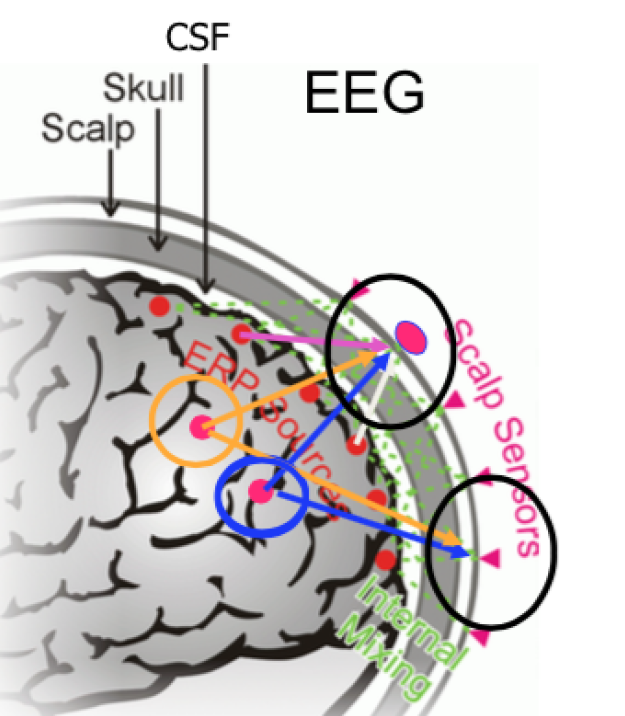
\includegraphics[width=\textwidth]{figurs/scalp.png}
        \caption{Illustration of volume conduction, source: \cite{phd2015}(we will make our own figure here instead)}\label{fig:volumeconduction}
    \end{minipage} 
    \hfill
    \begin{minipage}[t]{.45\textwidth}
        \centering
        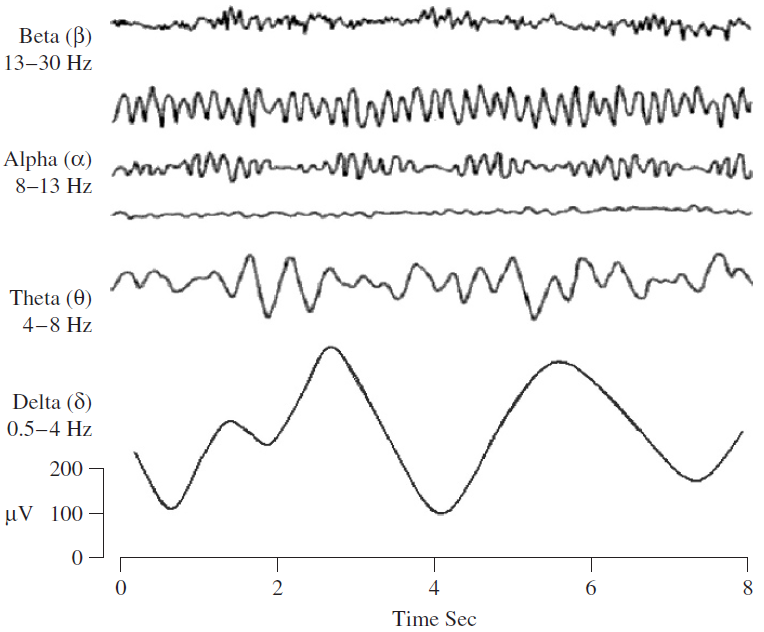
\includegraphics[width=\textwidth]{figurs/EEG_example.png}
        \caption{Example of time dependent EEG measurements within the four defined categories, source: \cite{EEGsignalprocessing}}\label{fig:EEG_example}
    \end{minipage}
\end{figure}
\noindent
EEG performed on humans and animals have a great number of applications with both clinical and research purposes. 
Examples of clinical applications covers diagnosis and management of neurological disorders such as epilepsy and monitor alertness regarding coma or brain death.
EEG capitalizes on the procedure being non-invasive and fast.
Neural activity can be measured within fractions of a second after a stimuli has been provided. 
These advantages contributes to the wide range of applications within research of the neural processes involved in or resulting from actions, emotions or  cognition. Today such neural research are use in many different fields\cite[p. 4]{fundamentalEEG}.
% such as neuromarketing, biofeedback(optimisation of learning) and brain computer interface.  
The hearing aid industry is one example where this research is highly prioritized. 
At Eriksholm research center, which is a part of the hearing aid manufacturer Oticon, cognitive hearing science is a research area within fast development \cite{Weberik}. 
One main purpose at Eriksholm is to make it possible for a hearing aid to identify the user-intended sound source from real time EEG measurements and thereby exclude noise from elsewhere \cite{Emina2019} \cite{Bech2018}. 
It is essentially the well known but unsolved cocktail problem which is sought improved by use of EEG. 
This is where EEG and occasionally so called in-ear EEG is interesting. In conjunction with the technology of beamforming it is possible for a hearing aid to receive only signals from a specific direction. 

Over the past two decades, functional integration has become an area of interest regarding EEG research \cite{Friston2011}. 
Within neurobiology functional integration refers to the study of the correlation among activities in different regions of the brain. 
In other words, how do different parts of the brain work together to process information and conduct a response \cite{Friston2002}.     
For this purpose separation and localization of the original sources which contribute to the EEG measurement is of interest. 
An article from 2016 \cite{Van2019} points out the importance of performing analysis regarding functional integration at source level rather than at EEG level. 
It is argued through experiments that analysis at EEG level does not allow interpretations about the interaction between sources. 
This emphasize a potential for improving results within a wide range of EEG research, if the original active sources can be extracted from a specific EEG measurements.    

     
%However, the focus of this research is the correlation between EEG measurements and the sound source rather than localization of the activated source from the EEG \cite{Emina2019}. 
%Hence a source localization approach could potentially be of interest regarding hearing aids in order to improve the results.
%(Furthermore, a real-time application to provide feedback from EEG measurements would be essential.)\todo{?}. 


\section{Modelling}
Consider the issue of extracting the activated sources from EEG measurements. A known approach is to model the observed data by the following linear system 
\begin{align*}
\mathbf{Y} = \mathbf{AX}.
\end{align*}
$\mathbf{Y} \in \mathbb{R}^{M \times L}$ is the EEG measurements where $L$ is the number of samples over time with each sample consisting of $M$ measurements, one for each sensor. $\mathbf{X} \in \mathbb{R}^{N \times L}$ makes $L$ samples of $N$ possible sources within the brain. The non-zero entries of a column in $\textbf{X}$ represent the active sources at the time of the sample. $\mathbf{A} \in \mathbb{R}^{M \times N}$ is an unknown mixing matrix. 
The $i^{th}$ column of $\mathbf{A}$ represents the relative projection weights from the $i^{th}$ source to every sensor \cite{phd2015}. 
This is in general referred to as a multiple measurement vector model. 
The aim in this case is to identify both $\mathbf{A}$ and $\mathbf{X}$ given the measurements $\mathbf{Y}$. 
This specific set up is referred to as the EEG inverse problem.  
\todo{her burde vi rise dictionarylearning of alm løsning af ligning system op}
To solve the EEG inverse problem the concept of sparse signal recovery makes a solid foundation, including compressive sensing and dictionary learning. 
Independent Component Analysis (ICA) is a commonly applied method to solve the inverse problem \cite{Scott1996}, \cite{Scott1997}. Here statistical independence between the active sources is the essential assumption. 
\\
Application of ICA has shown great results regarding source separation of high-density EEG. 
%Furthermore, an enhanced signal-to-noise ratio of the unmixed independent source time series processes allow essential study of the behaviour and relationships between multiple EEG source processes \cite{Arnaud2012}. 
However, a significant flaw to this method is that the EEG measurements are only separated into a number of sources that are equal to or less than the number of sensors \cite{Balkan2015}.
This means that the EEG inverse problem may not form an under-determined system, which is the case when the number of unknown sources exceeds the number of sensors. 
That is an assumption which undermines the reliability and usability of ICA, as the number of simultaneous active sources easily exceed the number of sensors \cite{phd2015}. 
This is especially a drawback when low-density EEG are considered. Low-density EEG measurements are collected from equipment with less than 32 sensors. 
However, improved capabilities of low-density EEG devices are desirable due to their relative low cost, mobility and ease to use. 
\\
The above argumentation gives rise to further investigation of existing work considering the under-determined inverse EEG problem. 

\section{Related Work and Our Contribution} 
As mentioned above ICA has been a solid method for source localization in the case where a separation into a number of sources equal to the number of sensors was adequate. The issue occurs in cases where the number of sources $N$ exceeds the number of sensors $M$.  
To overcome this issue an extension of ICA was suggested, referred to as the ICA mixture model \cite{Balkan2015}.
Instead of identifying one overcomplete mixing matrix $\mathbf{A} \in \mathbb{R}^{M \times N}$ this approach learns $N_{\text{model}}$ different mixing matrices $\mathbf{A}_i \in \mathbb{R}^{M\times M}$, to make computations more tractable. 
The method was further adapted into the Adaptive Mixture ICA (AMICA) which showed successful results regarding identification of more sources than available sensors \cite{Palmer2008}. 
However, the successful results relies on the assumption that no more than $M$ sources is simultaneously active. This assumption is still an essential limitation to the frame work, especially when considering low-density EEG. 
Other types of overcomplete ICA algorithms have been proposed to overcome the problem of learning over-complete systems. 
One is the Restricted ICA (RICA), an efficient method used for unsupervised learning in neural networks \cite{Le2011}.\\ 

In 2015 O. Balkan et. al., \cite{Balkan2015}, suggested a new approach also targeting the identification of more sources than sensors regarding EEG. 
The suggested method, referred to as Cov-DL, is a covariance-domain based dictionary learning algorithm. 
The point is to transfer the EEG measurements into the covariance domain, for which higher dimensionality can be achieved compared to the original EEG sensor domain of size $M$. 
This transformation can be done when assuming the scalp mixing is linear and under the assumption of no correlation between the sources within a certain time-window. 
The Cov-DL algorithm stands out from the other straight forward dictionary learning methods as it does not relay on the sparsity of active sources. This is an essential advantage when low-density EEG is considered. 
Cov-DL was tested and found to outperform both AMICA and RICA \cite{Balkan2015}. Thus it is considered the state of the art within the area of source recovery. 
\\ \\
It is essential to note that the Cov-DL algorithm only learns the mixing matrix $\mathbf{A}$, the projection of sources to the scalp sensors, and not the explicit source activity time series $\mathbf{X}$.
\\
For purpose of recovering $\textbf{X}$, from $\textbf{Y}$ and $\textbf{A}$ found by Cov-DL, a multiple measurement sparse Bayesian learning (M-SBL) algorithm was proposed in \cite{Balkan2014} by O. Balkan et. al. This methos is also targeting the case of more active sources than sensors. 
The method was proven to outperform the previously used algorithm, even when the defined recovery conditions regarding the found mixing matrix $\textbf{A}$ was not fulfilled\cite{Balkan2014}.  
\\ \\
The two state of the art methods for source recovery makes the foundation of this thesis. 
This thesis proposes an algorithm with the purpose of solving the EEG inverse problem using the presented methods on EEG measurements. 
To extend the existing results the algorithm is expanded into a real-time application, in order to provide feedback based on the source activity.
\\
The intention of the feedback is to allow a hearing aid to react when the user is using an unnecessary amount of energy in order to listen to some signal which could be dominated by noise. Here the amount of energy is based on the number of active sources within the brain. A reaction from the hearing aid could be to adjust the direction of the microphone beam within the hearing aid.    
For this, the application is tested within a simulation environment where the receiving direction of the test person can be adjusted in real-time. 
The quality of the final results is measured by the capability of improving the listener experience and the time used to provide useful feedback. 
\\ \\
As such our contribution \textit{(hopefully)} consists of tests of existing methods on real-time measurements and furthermore include a feedback to control the microphone beam on a hearing aid. \todo{note: Evt. kunne vi lave en figur der lidt ala mindmap sætte et system overblik op og så highlighte de "bokse" vi vælger at arbejde med.}
